\documentclass[11pt,fleqn]{book} % Default font size and left-justified equations

%%%%%%%%%%%%%%%%%%%%%%%%%%%%%%%%%%%%%%%%%
% The Legrand Orange Book
% Structural Definitions File
% Version 2.1 (26/09/2018)
%
% Original author:
% Mathias Legrand (legrand.mathias@gmail.com) with modifications by:
% Vel (vel@latextemplates.com)
% 
% This file was downloaded from:
% http://www.LaTeXTemplates.com
%
% License:
% CC BY-NC-SA 3.0 (http://creativecommons.org/licenses/by-nc-sa/3.0/)
%
%%%%%%%%%%%%%%%%%%%%%%%%%%%%%%%%%%%%%%%%%

%----------------------------------------------------------------------------------------
%	VARIOUS REQUIRED PACKAGES AND CONFIGURATIONS
%----------------------------------------------------------------------------------------

\usepackage[table]{xcolor}

\usepackage{graphicx}
\usepackage{tabularx} % Required for including pictures
\usepackage{pgf,tikz,tkz-tab,eurosym,yhmath, stmaryrd}
\usepackage{pgfplots}
\usepackage{mathrsfs}
\usetikzlibrary{patterns}
\usetikzlibrary{trees}
\graphicspath{{../../Pictures/}}
\usepackage{multicol} 


\usepackage[english]{babel} % English language/hyphenation
\usepackage{icomma}
\usepackage{enumitem} % Customize lists
\setlist{nolistsep, nosep, nolistsep} % Reduce spacing between bullet points and numbered lists

\usepackage{booktabs} % Required for nicer horizontal rules in tables

 % Required for specifying colors by name


\definecolor{ocre}{RGB}{243,102,25} % Define the orange color used for highlighting throughout the book

\usepackage{listings}

\definecolor{codegreen}{rgb}{0,0.6,0}
\definecolor{codegray}{rgb}{0.5,0.5,0.5}
\definecolor{codepurple}{rgb}{0.58,0,0.82}
\definecolor{backcolour}{rgb}{0.95,0.95,0.92}

\lstdefinestyle{mystyle}{
    backgroundcolor=\color{backcolour},   
    commentstyle=\color{codegreen},
    keywordstyle=\color{magenta},
    numberstyle=\tiny\color{codegray},
    stringstyle=\color{codepurple},
    basicstyle=\ttfamily\footnotesize,
    breakatwhitespace=false,         
    breaklines=true,                 
    captionpos=b,                    
    keepspaces=true,                 
    numbers=left,                    
    numbersep=5pt,                  
    showspaces=false,                
    showstringspaces=false,
    showtabs=false,                  
    tabsize=2
}

\lstset{style=mystyle}

%----------------------------------------------------------------------------------------
% Paramétrage XSIM
%----------------------------------------------------------------------------------------

\usepackage[no-files]{xsim}


\DeclareExerciseEnvironmentTemplate{myex}{%
    \textbf{%
      \hypertarget{ex:\ExerciseID}{\sffamily{\ensuremath{\blacktriangleright}} Exercice \GetExerciseProperty{counter} \GetExerciseProperty{subtitle} --}
      \hyperlink{sol:\ExerciseID}{Voir le corrigé}%
    }\par
}{\par\smallskip}

\DeclareExerciseEnvironmentTemplate{mysol}{%
    \textbf{%
      \hypertarget{sol:\ExerciseID}{\sffamily{\ensuremath{\blacktriangleright}} Correction \GetExerciseProperty{counter} --}
      \hyperlink{ex:\ExerciseID}{Voir l'énoncé}%
    }\par
}{\par\medskip}

\xsimsetup{
  exercise/template = myex ,
  solution/template = mysol 
}

%Collection exercices

\DeclareExerciseTagging{topic}

\xsimsetup{collect}

%----------------------------------------------------------------------------------------
% SYMBOLES
%----------------------------------------------------------------------------------------

\newcommand\imCMsym[4][\mathord]{%
  \DeclareFontFamily{U} {#2}{}
  \DeclareFontShape{U}{#2}{m}{n}{
    <-6> #25
    <6-7> #26
    <7-8> #27
    <8-9> #28
    <9-10> #29
    <10-12> #210
    <12-> #212}{}
  \DeclareSymbolFont{CM#2} {U} {#2}{m}{n}
  \DeclareMathSymbol{#4}{#1}{CM#2}{#3}
}
\newcommand\alsoimCMsym[4][\mathord]{\DeclareMathSymbol{#4}{#1}{CM#2}{#3}}

\imCMsym{cmmi}{124}{\CMjmath}

\newcommand{\Oij}{(O\,;\,\vec{\imath}\,,\, \vec{\CMjmath} )}
\newcommand{\Oijk}{(O\,;\,\vec{\imath}\,,\, \vec{\CMjmath}\,,\,\vec{k})}

\newcommand\e{\mathrm{e}}
\newcommand\R{\mathbb{R}}
\newcommand\N{\mathbb{N}}


%----------------------------------------------------------------------------------------
%	MARGINS
%----------------------------------------------------------------------------------------

\usepackage{geometry} % Required for adjusting page dimensions and margins

\geometry{
	paper=a4paper, % Paper size, change to letterpaper for US letter size
	top=3cm, % Top margin
	bottom=3cm, % Bottom margin
	left=2cm, % Left margin
	right=2cm, % Right margin
	headheight=14pt, % Header height
	footskip=1.4cm, % Space from the bottom margin to the baseline of the footer
	headsep=10pt, % Space from the top margin to the baseline of the header
	%showframe, % Uncomment to show how the type block is set on the page
}

\setlength{\parindent}{0pt}
\parskip=5pt



%----------------------------------------------------------------------------------------
%	FONTS
%----------------------------------------------------------------------------------------

\usepackage{avant} % Use the Avantgarde font for headings
\usepackage{times} % Use the Times font for headings
\usepackage{mathptmx} % Use the Adobe Times Roman as the default text font together with math symbols from the Sym­bol, Chancery and Com­puter Modern fonts

%\usepackage{microtype} % Slightly tweak font spacing for aesthetics
%\usepackage[utf8]{inputenc} % Required for including letters with accents
\usepackage[T1]{fontenc} % Use 8-bit encoding that has 256 glyphs

%----------------------------------------------------------------------------------------
%	BIBLIOGRAPHY AND INDEX
%----------------------------------------------------------------------------------------

\usepackage[style=numeric,citestyle=numeric,sorting=nyt,sortcites=true,autopunct=true,babel=hyphen,hyperref=true,abbreviate=false,backref=true,backend=biber]{biblatex}
\addbibresource{bibliography.bib} % BibTeX bibliography file
\defbibheading{bibempty}{}

\usepackage{calc} % For simpler calculation - used for spacing the index letter headings correctly
\usepackage{makeidx} % Required to make an index
\makeindex % Tells LaTeX to create the files required for indexing

%----------------------------------------------------------------------------------------
%	MAIN TABLE OF CONTENTS
%----------------------------------------------------------------------------------------

\usepackage{titletoc} % Required for manipulating the table of contents

\contentsmargin{0cm} % Removes the default margin

% Part text styling (this is mostly taken care of in the PART HEADINGS section of this file)
\titlecontents{part}
	[0cm] % Left indentation
	{\addvspace{20pt}\bfseries} % Spacing and font options for parts
	{}
	{}
	{}

% Chapter text styling
\titlecontents{chapter}
	[1.25cm] % Left indentation
	{\addvspace{12pt}\large\sffamily\bfseries} % Spacing and font options for chapters
	{\color{ocre!60}\contentslabel[\Large\thecontentslabel]{1.25cm}\color{ocre}} % Formatting of numbered sections of this type
	{\color{ocre}} % Formatting of numberless sections of this type
	{\color{ocre!60}\normalsize\;\titlerule*[.5pc]{.}\;\thecontentspage} % Formatting of the filler to the right of the heading and the page number

% Section text styling
\titlecontents{section}
	[1.25cm] % Left indentation
	{\addvspace{3pt}\sffamily\bfseries} % Spacing and font options for sections
	{\contentslabel[\thecontentslabel]{1.25cm}} % Formatting of numbered sections of this type
	{} % Formatting of numberless sections of this type
	{\hfill\color{black}\thecontentspage} % Formatting of the filler to the right of the heading and the page number

% Subsection text styling
\titlecontents{subsection}
	[1.25cm] % Left indentation
	{\addvspace{1pt}\sffamily\small} % Spacing and font options for subsections
	{\contentslabel[\thecontentslabel]{1.25cm}} % Formatting of numbered sections of this type
	{} % Formatting of numberless sections of this type
	{\ \titlerule*[.5pc]{.}\;\thecontentspage} % Formatting of the filler to the right of the heading and the page number

% Figure text styling
\titlecontents{figure}
	[1.25cm] % Left indentation
	{\addvspace{1pt}\sffamily\small} % Spacing and font options for figures
	{\thecontentslabel\hspace*{1em}} % Formatting of numbered sections of this type
	{} % Formatting of numberless sections of this type
	{\ \titlerule*[.5pc]{.}\;\thecontentspage} % Formatting of the filler to the right of the heading and the page number

% Table text styling
\titlecontents{table}
	[1.25cm] % Left indentation
	{\addvspace{1pt}\sffamily\small} % Spacing and font options for tables
	{\thecontentslabel\hspace*{1em}} % Formatting of numbered sections of this type
	{} % Formatting of numberless sections of this type
	{\ \titlerule*[.5pc]{.}\;\thecontentspage} % Formatting of the filler to the right of the heading and the page number

%----------------------------------------------------------------------------------------
%	MINI TABLE OF CONTENTS IN PART HEADS
%----------------------------------------------------------------------------------------

% Chapter text styling
\titlecontents{lchapter}
	[0em] % Left indentation
	{\addvspace{15pt}\large\sffamily\bfseries} % Spacing and font options for chapters
	{\color{ocre}\contentslabel[\Large\thecontentslabel]{1.25cm}\color{ocre}} % Chapter number
	{}  
	{\color{ocre}\normalsize\sffamily\bfseries\;\titlerule*[.5pc]{.}\;\thecontentspage} % Page number

% Section text styling
\titlecontents{lsection}
	[0em] % Left indentation
	{\sffamily\small} % Spacing and font options for sections
	{\contentslabel[\thecontentslabel]{1.25cm}} % Section number
	{}
	{}

% Subsection text styling (note these aren't shown by default, display them by searchings this file for tocdepth and reading the commented text)
\titlecontents{lsubsection}
	[.5em] % Left indentation
	{\sffamily\footnotesize} % Spacing and font options for subsections
	{\contentslabel[\thecontentslabel]{1.25cm}}
	{}
	{}

%----------------------------------------------------------------------------------------
%	HEADERS AND FOOTERS
%----------------------------------------------------------------------------------------


\usepackage{fancyhdr} % Required for header and footer configuration

\pagestyle{fancy}
\renewcommand{\chaptermark}[1]{\markboth{\sffamily\normalsize\bfseries\ \thechapter.\ #1}{}} % Chapter text font settings
\renewcommand{\sectionmark}[1]{\markright{\sffamily\normalsize\thesection\hspace{5pt}#1}{}} % Section text font settings
\fancyhf{} \fancyhead[LE,RO]{\sffamily\normalsize\thepage} % Font setting for the page number in the header
\fancyhead[LO]{\rightmark} % Print the nearest section name on the left side of odd pages
\fancyhead[RE]{\leftmark} % Print the current chapter name on the right side of even pages

\fancyfoot[L]{Jason LAPEYRONNIE}
\fancyfoot[R]{\href{http://mathoutils.fr}{http://mathoutils.fr}} % Uncomment to include a footer

\renewcommand{\headrulewidth}{0.5pt} % Thickness of the rule under the header
\renewcommand{\footrulewidth}{0.5pt} % Thickness of the rule under the header

\fancypagestyle{plain}{% Style for when a plain pagestyle is specified
	\fancyhead{}\renewcommand{\headrulewidth}{0pt}%
}

% Removes the header from odd empty pages at the end of chapters
\makeatletter
\renewcommand{\cleardoublepage}{
\clearpage\ifodd\c@page\else
\hbox{}
\vspace*{\fill}
\thispagestyle{empty}
\newpage
\fi}

%----------------------------------------------------------------------------------------
%	THEOREM STYLES
%----------------------------------------------------------------------------------------

\usepackage{amsmath,amsfonts,amssymb,amsthm} % For math equations, theorems, symbols, etc

\newcommand{\intoo}[2]{\mathopen{]}#1\,;#2\mathclose{[}}
\newcommand{\ud}{\mathop{\mathrm{{}d}}\mathopen{}}
\newcommand{\intff}[2]{\mathopen{[}#1\,;#2\mathclose{]}}
\renewcommand{\qedsymbol}{$\blacksquare$}
\newtheorem{notation}{Notation}[section]

% Boxed/framed environments
\newtheoremstyle{ocrenumbox}% Theorem style name
{0pt}% Space above
{0pt}% Space below
{\normalfont}% Body font
{}% Indent amount
{\small\bf\sffamily\color{ocre}}% Theorem head font
{\;:\;}% Punctuation after theorem head
{0.25em}% Space after theorem head
{\small\sffamily\color{ocre}\thmname{#1}\nobreakspace\thmnumber{\@ifnotempty{#1}{}\@upn{#2}}% Theorem text (e.g. Theorem 2.1)
\thmnote{\nobreakspace\the\thm@notefont\sffamily\bfseries\color{black}---\nobreakspace#3}} % Optional theorem note

\newtheoremstyle{blacknumex}% Theorem style name
{5pt}% Space above
{10pt}% Space below
{\normalfont}% Body font
{} % Indent amount
{\small\bf\sffamily}% Theorem head font
{\;:\;}% Punctuation after theorem head
{0.25em}% Space after theorem head
{\small\sffamily{\tiny\ensuremath{\blacksquare}}\nobreakspace\thmname{#1}\nobreakspace\thmnumber{\@ifnotempty{#1}{}\@upn{#2}}% Theorem text (e.g. Theorem 2.1)
\thmnote{\nobreakspace\the\thm@notefont\sffamily\bfseries---\nobreakspace#3}}% Optional theorem note

\newtheoremstyle{blacknumexo}% Theorem style name
{15pt}% Space above
{10pt}% Space below
{\normalfont}% Body font
{} % Indent amount
{\small\bf\sffamily}% Theorem head font
{}% Punctuation after theorem head
{0.5em}% Space after theorem head
{\small\sffamily{\ensuremath{\blacktriangleright}}\nobreakspace\thmname{#1}\nobreakspace\thmnumber{\@ifnotempty{#1}{}\@upn{#2}}% Theorem text (e.g. Theorem 2.1)
\thmnote{\nobreakspace\the\thm@notefont\sffamily\bfseries---\nobreakspace#3} \\}% Optional theorem note



\newtheoremstyle{blacknumbox} % Theorem style name
{0pt}% Space above
{5pt}% Space below
{}% Body font
{}% Indent amount
{\large\bf\sffamily}% Theorem head font
{\;:\;}% Punctuation after theorem head
{0.25em}% Space after theorem head
{\small\sffamily\thmname{#1}\nobreakspace\thmnumber{\@ifnotempty{#1}{}\@upn{#2}}% Theorem text (e.g. Theorem 2.1)
\thmnote{\nobreakspace\the\thm@notefont\sffamily\bfseries---\nobreakspace#3}}% Optional theorem note

% Non-boxed/non-framed environments
\newtheoremstyle{ocrenum}% Theorem style name
{5pt}% Space above
{5pt}% Space below
{\normalfont}% Body font
{}% Indent amount
{\small\bf\sffamily\color{ocre}}% Theorem head font
{\;:\;}% Punctuation after theorem head
{0.25em}% Space after theorem head
{\small\sffamily\color{ocre}\thmname{#1}\nobreakspace\thmnumber{\@ifnotempty{#1}{}\@upn{#2}}% Theorem text (e.g. Theorem 2.1)
\thmnote{\nobreakspace\the\thm@notefont\sffamily\bfseries\color{black}---\nobreakspace#3}} % Optional theorem note
\makeatother

% Defines the theorem text style for each type of theorem to one of the three styles above
\newcounter{dummy} 
\newcounter{thm}
\newcounter{correction}
\newcounter{qst}
\theoremstyle{ocrenumbox}
\newtheorem{theoremeT}[dummy]{Théorème}
\newtheorem{exerciseT}{Propriété}
\newtheorem{principeT}{Principe}
\theoremstyle{blacknumex}
\newtheorem{exampleT}{Exemple}
\theoremstyle{blacknumexo}
\newtheorem{exo}[thm]{Exercice}
\newtheorem{corr}[correction]{Correction}
\newtheorem{quest}[qst]{Question}
\theoremstyle{blacknumbox}
\newtheorem{vocabulary}{Vocabulary}[section]
\newtheorem{definitionT}{Définition}
\newtheorem{corollaryT}[dummy]{Corollary}
\theoremstyle{ocrenum}
\newtheorem{proofT}[dummy]{Démonstration}


%----------------------------------------------------------------------------------------
%	DEFINITION OF COLORED BOXES
%----------------------------------------------------------------------------------------

\RequirePackage[framemethod=default]{mdframed} % Required for creating the theorem, definition, exercise and corollary boxes

% Theorem box
\newmdenv[skipabove=7pt,
skipbelow=7pt,
backgroundcolor=black!5,
linecolor=ocre,
innerleftmargin=5pt,
innerrightmargin=5pt,
innertopmargin=10pt,
leftmargin=0cm,
rightmargin=0cm,
innerbottommargin=5pt]{tBox}

%Proposition box	  
\newmdenv[skipabove=7pt,
skipbelow=7pt,
rightline=false,
leftline=true,
topline=false,
bottomline=false,
backgroundcolor=ocre!10,
linecolor=ocre,
innerleftmargin=5pt,
innerrightmargin=5pt,
innertopmargin=10pt,
innerbottommargin=3pt,
leftmargin=0cm,
rightmargin=0cm,
linewidth=4pt]{eBox}	

% Definition box
\newmdenv[skipabove=7pt,
backgroundcolor=ocre!4,
skipbelow=7pt,
rightline=false,
leftline=true,
topline=false,
bottomline=false,
linecolor=ocre,
innerleftmargin=5pt,
innerrightmargin=5pt,
innertopmargin=10pt,
leftmargin=0cm,
rightmargin=0cm,
linewidth=4pt,
innerbottommargin=5pt]{dBox}	

% Corollary box
\newmdenv[skipabove=7pt,
skipbelow=7pt,
rightline=false,
leftline=true,
topline=false,
bottomline=false,
linecolor=gray,
backgroundcolor=black!5,
innerleftmargin=5pt,
innerrightmargin=5pt,
innertopmargin=5pt,
leftmargin=0cm,
rightmargin=0cm,
linewidth=4pt,
innerbottommargin=5pt]{cBox}

\newmdenv[skipabove=7pt,
skipbelow=7pt,
backgroundcolor=black!5,
innerleftmargin=5pt,
topline=false,
bottomline=false,
rightline=false,
leftline=false,
innerrightmargin=5pt,
innertopmargin=5pt,
leftmargin=0cm,
rightmargin=0cm,
innerbottommargin=5pt]{xBox}

% Creates an environment for each type of theorem and assigns it a theorem text style from the "Theorem Styles" section above and a colored box from above
\newenvironment{theorem}{\begin{tBox}\begin{theoremeT}}{\end{theoremeT}\end{tBox}}

\newenvironment{exo2}{\noindent \begin{exo}\item\relax \noindent \begin{eBox}\item\relax}{\end{eBox}\end{exo}}


\newenvironment{proposition}{\begin{eBox}\begin{exerciseT}}{\hfill{\color{ocre}}\end{exerciseT}\end{eBox}}		

\newenvironment{principe}{\begin{eBox}\begin{principeT}}{\hfill{\color{ocre}}\end{principeT}\end{eBox}}	
		  
\newenvironment{definition}{\begin{dBox}\begin{definitionT}}{\end{definitionT}\end{dBox}}	

\newenvironment{example}{\begin{xBox}\begin{exampleT}}{\hfill{\tiny\ensuremath{\blacksquare}}\end{exampleT}\end{xBox}}

\newenvironment{demonstration}{\begin{proofT}}{\hfill{\tiny\ensuremath{\square}}\end{proofT}}		
\newenvironment{corollary}{\begin{cBox}\begin{corollaryT}}{\end{corollaryT}\end{cBox}}	

%----------------------------------------------------------------------------------------
%	REMARK ENVIRONMENT
%----------------------------------------------------------------------------------------

\newenvironment{remark}{\par\vspace{5pt}\small % Vertical white space above the remark and smaller font size
\begin{list}{}{
\leftmargin=25pt % Indentation on the left
\rightmargin=15pt}\item\ignorespaces % Indentation on the right
\makebox[-2.5pt]{
\begin{tikzpicture}[overlay]
\node[draw=ocre!60,line width=1pt,circle,fill=ocre!25,font=\sffamily\bfseries,inner sep=2pt,outer sep=0pt] at (-15pt,0pt){\textcolor{ocre}{R}};\end{tikzpicture}} % Orange R in a circle
\advance\baselineskip -1pt}{\end{list}\vskip5pt} % Tighter line spacing and white space after remark

%----------------------------------------------------------------------------------------
%	SECTION NUMBERING IN THE MARGIN
%----------------------------------------------------------------------------------------

\makeatletter
\renewcommand{\@seccntformat}[1]{\llap{\textcolor{ocre}{\csname the#1\endcsname}\hspace{1em}}}                    
\renewcommand{\section}{\@startsection{section}{1}{\z@}
{-4ex \@plus -1ex \@minus -.4ex}
{1ex \@plus.2ex }
{\normalfont\LARGE\sffamily\bfseries}}
\renewcommand{\subsection}{\@startsection {subsection}{2}{\z@}
{-3ex \@plus -0.1ex \@minus -.4ex}
{0.5ex \@plus.2ex }
{\normalfont\sffamily\bfseries}}
\renewcommand{\subsubsection}{\@startsection {subsubsection}{3}{\z@}
{-2ex \@plus -0.1ex \@minus -.2ex}
{.2ex \@plus.2ex }
{\normalfont\small\sffamily\bfseries}}                        
\renewcommand\paragraph{\@startsection{paragraph}{4}{\z@}
{-2ex \@plus-.2ex \@minus .2ex}
{.1ex}
{\normalfont\small\sffamily\bfseries}}

%----------------------------------------------------------------------------------------
%	PART HEADINGS
%----------------------------------------------------------------------------------------

% Numbered part in the table of contents
\newcommand{\@mypartnumtocformat}[2]{%
	\setlength\fboxsep{0pt}%
	\noindent\colorbox{ocre!20}{\strut\parbox[c][.7cm]{\ecart}{\color{ocre!70}\Large\sffamily\bfseries\centering#1}}\hskip\esp\colorbox{ocre!40}{\strut\parbox[c][.7cm]{\linewidth-\ecart-\esp}{\Large\sffamily\centering#2}}%
}

% Unnumbered part in the table of contents
\newcommand{\@myparttocformat}[1]{%
	\setlength\fboxsep{0pt}%
	\noindent\colorbox{ocre!40}{\strut\parbox[c][.7cm]{\linewidth}{\Large\sffamily\centering#1}}%
}

\newlength\esp
\setlength\esp{4pt}
\newlength\ecart
\setlength\ecart{1.2cm-\esp}
\newcommand{\thepartimage}{}%
\newcommand{\partimage}[1]{\renewcommand{\thepartimage}{#1}}%
\def\@part[#1]#2{%
\ifnum \c@secnumdepth >-2\relax%
\refstepcounter{part}%
\addcontentsline{toc}{part}{\texorpdfstring{\protect\@mypartnumtocformat{\thepart}{#1}}{\partname~\thepart\ ---\ #1}}
\else%
\addcontentsline{toc}{part}{\texorpdfstring{\protect\@myparttocformat{#1}}{#1}}%
\fi%
\startcontents%
\markboth{}{}%
{\thispagestyle{empty}%
\begin{tikzpicture}[remember picture,overlay]%
\node at (current page.north west){\begin{tikzpicture}[remember picture,overlay]%	
\fill[ocre!20](0cm,0cm) rectangle (\paperwidth,-\paperheight);
\node[anchor=north] at (4cm,-3.25cm){\color{ocre!40}\fontsize{220}{100}\sffamily\bfseries\thepart}; 
\node[anchor=south east] at (\paperwidth-1cm,-\paperheight+1cm){\parbox[t][][t]{8.5cm}{
\printcontents{l}{0}{\setcounter{tocdepth}{1}}% The depth to which the Part mini table of contents displays headings; 0 for chapters only, 1 for chapters and sections and 2 for chapters, sections and subsections
}};
\node[anchor=north east] at (\paperwidth-1.5cm,-3.25cm){\parbox[t][][t]{15cm}{\strut\raggedleft\color{white}\fontsize{30}{30}\sffamily\bfseries#2}};
\end{tikzpicture}};
\end{tikzpicture}}%
\@endpart}
\def\@spart#1{%
\startcontents%
\phantomsection
{\thispagestyle{empty}%
\begin{tikzpicture}[remember picture,overlay]%
\node at (current page.north west){\begin{tikzpicture}[remember picture,overlay]%	
\fill[ocre!20](0cm,0cm) rectangle (\paperwidth,-\paperheight);
\node[anchor=north east] at (\paperwidth-1.5cm,-3.25cm){\parbox[t][][t]{15cm}{\strut\raggedleft\color{white}\fontsize{30}{30}\sffamily\bfseries#1}};
\end{tikzpicture}};
\end{tikzpicture}}
\addcontentsline{toc}{part}{\texorpdfstring{%
\setlength\fboxsep{0pt}%
\noindent\protect\colorbox{ocre!40}{\strut\protect\parbox[c][.7cm]{\linewidth}{\Large\sffamily\protect\centering #1\quad\mbox{}}}}{#1}}%
\@endpart}
\def\@endpart{\vfil\newpage
\if@twoside
\if@openright
\null
\thispagestyle{empty}%
\newpage
\fi
\fi
\if@tempswa
\twocolumn
\fi}

%----------------------------------------------------------------------------------------
%	CHAPTER HEADINGS
%----------------------------------------------------------------------------------------

% A switch to conditionally include a picture, implemented by Christian Hupfer
\newif\ifusechapterimage
\usechapterimagetrue
\newcommand{\thechapterimage}{}%
\newcommand{\chapterimage}[1]{\ifusechapterimage\renewcommand{\thechapterimage}{#1}\fi}%
\newcommand{\autodot}{.}
\def\@makechapterhead#1{%
{\parindent \z@ \raggedright \normalfont
\ifnum \c@secnumdepth >\m@ne
\if@mainmatter
\begin{tikzpicture}[remember picture,overlay]
\node at (current page.north west)
{\begin{tikzpicture}[remember picture,overlay]
\node[anchor=north west,inner sep=0pt] at (0,0) {\ifusechapterimage\includegraphics[width=\paperwidth]{\thechapterimage}\fi};
\draw[anchor=west] (\Gm@lmargin,-3cm) node [line width=2pt,rounded corners=15pt,draw=ocre,fill=white,fill opacity=0.5,inner sep=15pt]{\strut\makebox[22cm]{}};
\draw[anchor=west] (\Gm@lmargin+.3cm,-3cm) node {\huge\sffamily\bfseries\color{black}\thechapter\autodot~#1\strut};
\end{tikzpicture}};
\end{tikzpicture}
\else
\begin{tikzpicture}[remember picture,overlay]
\node at (current page.north west)
{\begin{tikzpicture}[remember picture,overlay]
\node[anchor=north west,inner sep=0pt] at (0,0) {\ifusechapterimage\includegraphics[width=\paperwidth]{\thechapterimage}\fi};
\draw[anchor=west] (\Gm@lmargin,-3cm) node [line width=2pt,rounded corners=15pt,draw=ocre,fill=white,fill opacity=0.5,inner sep=15pt]{\strut\makebox[22cm]{}};
\draw[anchor=west] (\Gm@lmargin+.3cm,-3cm) node {\huge\sffamily\bfseries\color{black}#1\strut};
\end{tikzpicture}};
\end{tikzpicture}
\fi\fi\par\vspace*{50\p@}}}

%-------------------------------------------

\def\@makeschapterhead#1{%
\begin{tikzpicture}[remember picture,overlay]
\node at (current page.north west)
{\begin{tikzpicture}[remember picture,overlay]
\node[anchor=north west,inner sep=0pt] at (0,0) {\ifusechapterimage\includegraphics[width=\paperwidth]{\thechapterimage}\fi};
\draw[anchor=west] (\Gm@lmargin,-3cm) node [line width=2pt,rounded corners=15pt,draw=ocre,fill=white,fill opacity=0.5,inner sep=15pt]{\strut\makebox[22cm]{}};
\draw[anchor=west] (\Gm@lmargin+.3cm,-3cm) node {\huge\sffamily\bfseries\color{black}#1\strut};
\end{tikzpicture}};
\end{tikzpicture}
\par\vspace*{50\p@}}
\makeatother

%----------------------------------------------------------------------------------------
%	LINKS
%----------------------------------------------------------------------------------------

\usepackage{hyperref}
\hypersetup{hidelinks,backref=true,pagebackref=true,hyperindex=true,colorlinks=false,breaklinks=true,urlcolor=ocre,bookmarks=true,bookmarksopen=false}

\usepackage{bookmark}
\bookmarksetup{
open,
numbered,
addtohook={%
\ifnum\bookmarkget{level}=0 % chapter
\bookmarksetup{bold}%
\fi
\ifnum\bookmarkget{level}=-1 % part
\bookmarksetup{color=ocre,bold}%
\fi
}
}

\renewcommand*\thesection{\arabic{section}}

\newcommand*{\coord}[3]{% 
  \ensuremath{\overrightarrow{#1}\, 
    \begin{pmatrix} 
      #2\\ 
      #3 
    \end{pmatrix}}}
    
  \newcommand*{\coordb}[2]{% 
  \ensuremath{ 
    \begin{pmatrix} 
      #1\\ 
      #2 
    \end{pmatrix}}}

\newcommand*{\coorde}[4]{% 
  \renewcommand{\arraystretch}{1}\ensuremath{\overrightarrow{#1}\, 
    \begin{pmatrix} 
      #2\\ 
      #3 \\
      #4
    \end{pmatrix}}}    
  \newcommand*{\coordbe}[3]{% 
 \renewcommand{\arraystretch}{1} \ensuremath{ 
    \begin{pmatrix} 
      #1\\ 
      #2 \\
      #3
    \end{pmatrix}}}  
    
\newcommand{\Card}{\mathrm{Card}}



\begin{document}

\chapterimage{../../Pictures/background}

\chapter{Exercices : Suites et récurrence}

\setcounter{section}{0}

\section*{Principe}


\begin{exercise}
Soit $r$ un réel. On rappelle qu'une suite $(u_n)$ est arithmétique de raison $r$ si pour tout $n\in\mathbb{N}$, $u_{n+1}=u_n+r$. \\ Soit donc $(u_n)$ une suite arithmétique de raison $r$.
\begin{enumerate}
\item Montrer par récurrence que pour tout entier naturel $n$, on a $u_n=u_0+rn$.
\item \textbf{Application :} On considère la suite $(u_n)$ arithmétique de premier terme $u_0=4$ et de raison $r=8$.
\begin{enumerate}
\item Exprimer $u_n$ en fonction de $n$ pour tout entier naturel $n$.
\item Calculer $u_{18}$ à l'aide de cette formule.
\end{enumerate}
\end{enumerate}
\end{exercise}
\begin{solution}
Pour tout entier naturel $n$, on considère la proposition $P(n)$ : « $u_n=u_0 + rn$ ».
\begin{itemize}
\item \textbf{Initialisation :} Pour $n=0$, on a bien $u_0+r \times 0=u_0$. $P(0)$ est vraie.
\item \textbf{Hérédité :} Soit $n\in\mathbb{N}$. Supposons que $P(n)$ est vraie, c'est-à-dire $u_n=u_0+rn$. Or, $u_{n+1}=u_n+r$. Ainsi, $u_{n+1}=u_0+rn+r=u_0+r(n+1)$. $P(n+1)$ est donc vraie.
\item \textbf{Conclusion :} $P(0)$ est vraie. $P$ est héréditaire. Par récurrence, $P(n)$ est vraie pour tout entier naturel $n$.
\end{itemize}
D'après la question 1, , pour tout entier naturel  $n$, on a $u_n=4+8n$. Ainsi, $u_{18}=4+8\times 18 = 144$.\end{solution}



\begin{exercise}
Soit $q$ un réel. On rappelle qu'une suite $(u_n)$ est géométrique de raison $q$ si pour tout $n\in\mathbb{N}$, $u_{n+1}=q\times u_n$. \\Soit donc $(u_n)$ une suite géométrique de raison $q$.
\begin{enumerate}
\item Montrer par récurrence que pour tout entier naturel $n$, $u_n=u_0 \times q^n$.
\item \textbf{Application :} On considère la suite $(u_n)$ géométrique de premier terme $u_0=3$ et de raison $q=-2$.
\begin{enumerate}
\item Exprimer $u_n$ en fonction de $n$ pour tout entier naturel $n$.
\item Calculer $u_{12}$ à l'aide de cette formule.
\end{enumerate}
\end{enumerate}\end{exercise}
\begin{solution}Pour tout entier naturel $n$, on considère la proposition $P(n)$ : « $u_n=u_0 \times q^n $ ».
\begin{itemize}
\item \textbf{Initialisation :} Pour $n=0$, on a bien $u_0 \times q^0=u_0 \times 1 = u_0$. $P(0)$ est vraie.
\item \textbf{Hérédité :} Soit $n\in\mathbb{N}$. Supposons que $P(n)$ est vraie, c'est-à-dire $u_n=u_0 \times q^n$. Or, $u_{n+1}=q\,u_n$. Ainsi, $u_{n+1}=q \times u_0 \times q^n=u_0 \times q^{n+1}$. $P(n+1)$ est donc vraie.
\item \textbf{Conclusion :} $P(0)$ est vraie. $P$ est héréditaire. Par récurrence, $P(n)$ est vraie pour tout entier naturel $n$.
\end{itemize}

D'après la question précédente, on a, pour tout  $n\in\mathbb{N}$, $u_n=3 \times (-2)^n$. Ainsi, $u_{12}=3 \times (-2)^{12}=12288$.\end{solution}




\begin{exercise}
On considère la suite $(u_n)$ telle que $u_0=12$ et pour tout entier naturel $n$, $u_{n+1}=3u_n-8$.\\ Montrer par récurrence que pour tout entier naturel $n$, on a  $u_n=4+8\times 3^n$.\end{exercise}
\begin{solution}Pour tout entier naturel $n$, on considère la proposition $P(n)$ : « $u_n=4+8\times 3^n$ ».
\begin{itemize}
\item \textbf{Initialisation :} Pour $n=0$, on a bien $4+8\times 3^0=4+8\times 1 = 12 = u_0$. $P(0)$ est vraie.
\item \textbf{Hérédité :} Soit $n\in\mathbb{N}$. Supposons que $P(n)$ est vraie, c'est-à-dire $u_n=4+8\times 3^n$. Or, $u_{n+1}=3u_n-8$. Ainsi, $u_{n+1}=3(4+8\times3^n)-8=3\times 4 +3\times 8 \times 3^n - 8 = 4 + 8 \times 3^{n+1}$. $P(n+1)$ est donc vraie.
\item \textbf{Conclusion :} $P(0)$ est vraie. $P$ est héréditaire. Par récurrence, $P(n)$ est vraie pour tout entier naturel $n$.
\end{itemize}\end{solution}




\begin{exercise}
On considère la suite \((u_n)\) définie par \(u_1=1\) et, pour tout entier naturel \(n\), \[u_{n+1}= \dfrac{u_n}{\sqrt{u_n^2+1}}.\]
\begin{enumerate}
 	\item Calculer \(u_2\) et \(u_3\)
 	\item Conjecturer une expression de \(u_n\) en fonction de \(n\) pour tout entier naturel non nul $n$.
 	\item Démontrer cette conjecture par récurrence.
\end{enumerate}\end{exercise}
\begin{solution}On a
\begin{itemize}\item \( u_2 = \dfrac{u_1}{\sqrt{u_1^2+1}}=\dfrac{1}{\sqrt{1^2+1}}=\dfrac{1}{\sqrt{2}}\).
 	\item \( u_3 = \dfrac{u_2}{\sqrt{u_2^2+1}}=\dfrac{\frac{1}{\sqrt{2}}}{\sqrt{\left(\frac{1}{\sqrt{2}}\right)^2+1}}=\dfrac{\frac{1}{\sqrt{2}}}{\sqrt{\frac{1}{2}+1}}=\dfrac{1}{\sqrt{2}} \times \dfrac{1}{\sqrt{\frac{3}{2}}} = \dfrac{1}{\sqrt{2}} \times \sqrt{\dfrac{2}{3}} = \dfrac{1}{\sqrt{3}}\).
\end{itemize}
Pour tout entier naturel non nul \(n\), on pose \(\mathcal{P}(n)\) : « \(u_n=\dfrac{1}{\sqrt{n}}\) ».
\begin{itemize}
\item \textbf{Initialisation} : \( \dfrac{1}{\sqrt{1}}=1=u_1\), \( \mathcal{P}(1) \) est vraie.
\item \textbf{Hérédité} : Soit \(n\in\mathbb{N}\setminus \{0\}\). Supposons que \( \mathcal{P}(n)\) est vraie. On a donc \(u_n=\dfrac{1}{\sqrt{n}}\).Or, $u_{n+1}= \dfrac{u_n}{\sqrt{u_n^2+1}}$. Ainsi,
\[u_{n+1}= \dfrac{\frac{1}{\sqrt{n}}}{\sqrt{\left(\frac{1}{\sqrt{n}}\right)^2+1}}=\dfrac{1}{\sqrt{n}} \times \dfrac{1}{\sqrt{\frac{1}{n}+1}}=\dfrac{1}{\sqrt{n}} \times \dfrac{1}{\sqrt{\frac{n+1}{n}}}=\dfrac{1}{\sqrt{n}} \times \sqrt{\dfrac{n}{n+1}} = \dfrac{1}{\sqrt{n+1}}.\]\( \mathcal{P}(n+1)\) est donc vraie.
\item \textbf{Conclusion} : \(\mathcal{P}(1)\) est vraie et \(\mathcal{P}\) est héréditaire. Par récurrence, \(\mathcal{P}(n)\) est vraie pour tout entier naturel non nul \(n\)
\end{itemize}\end{solution}


\begin{exercise}
On considère la suite \((u_n)\) définie par \(u_0=3\) et, pour tout entier naturel \(n\), \(u_{n+1}=\dfrac{u_n-2}{2u_n+5}\).

Montrer que pour tout entier naturel \(n\), on a \[u_n = \dfrac{9-8n}{3+8n}.\]\end{exercise}
\begin{solution}Pour tout entier naturel \(n\), on pose \(\mathcal{P}(n)\) : « \(u_n =\dfrac{9-8n}{3+8n}\) ».
\begin{itemize} \item \textbf{Initialisation} : On a \(\dfrac{9-8 \times 0}{3+8 \times 0}=\dfrac{9}{3}=3=u_0\). \(\mathcal{P}(0)\) est vraie.
\item\textbf{Hérédité :} Soit \(n\in\mathbb{N}\). Supposons que \(\mathcal{P}(n)\) est vraie, c'est-à-dire \(u_n =\dfrac{9-8n}{3+8n}\). On cherche à établir
\[u_{n+1}=\dfrac{9-8(n+1)}{3+8(n+1)}=\dfrac{9-8n-8}{3+8n+8}=\dfrac{1-8n}{11+8n}.\]
Or, \(u_{n+1}=\dfrac{u_n-2}{2u_n+5}\). Ainsi, $u_{n+1}=\dfrac{\dfrac{9-8n}{3+8n}-2}{2 \times \dfrac{9-8n}{3+8n} +5} = \dfrac{\dfrac{9-8n-2(3+8n)}{3+8n}}{\dfrac{2(9-8n)+5(3+8n)}{3+8n}}$.

On a alors
\[u_{n+1}=\dfrac{9-8n-2(3+8n)}{3+8n} \times \dfrac{3+8n}{2(9-8n)+5(3+8n)}=\dfrac{9-8n-2(3+8n)}{2(9-8n)+5(3+8n)}.\]
et donc
\[u_{n+1}=\dfrac{9-8n-6-16n}{18-16n+15+40n}=\dfrac{3-24n}{33+24n}.\]
En factorisant par 3, on obtient finalement $u_{n+1}=\dfrac{3(1-8n)}{3(11+8n)}=\dfrac{1-8n}{11+8n}$, qui est bien le résultat voulu. \(\mathcal{P}(n+1)\) est vraie.
\item \textbf{Conclusion} :  \(\mathcal{P}(0)\) est vraie, \(\mathcal{P}\) est héréditaire. D'après le principe de récurrence, \(\mathcal{P}(n)\) est vraie pour tout entier naturel \(n\).\end{itemize}\end{solution}


\begin{exercise}
Montrer par récurrence que, pour tout entier naturel non nul $n$, on a \[1+2+3+\ldots + n=\dfrac{n(n+1)}{2}.\] \end{exercise}
\begin{solution}Pour tout entier naturel non nul $n$, on note $\mathcal{P}(n)$ la proposition  « $1+2+3+\ldots + n=\dfrac{n(n+1)}{2}$ ».
\begin{itemize}
\item D'une part, la somme de tous les entiers entre 1 et 1 vaut évidemment 1. Par ailleurs, $\dfrac{1\times (1+1)}{2}=1$. $\mathcal{P}(1)$ est vraie.
\item Soit $n$ un entier naturel non nul. Supposons que $\mathcal{P}(n)$ est vraie. On a alors
\[1+2+3+\ldots +n+(n+1) = \dfrac{n(n+1)}{2}+n+1=\dfrac{n(n+1)}{2}+\dfrac{2(n+1)}{2}=\dfrac{(n+1)(n+2)}{2}.\]
$\mathcal{P}(n+1)$ est donc vraie.
\item $\mathcal{P}(1)$ est vraie, $P$ est héréditaire. Par récurrence, $\mathcal{P}(n)$ est vraie pour tout entier naturel non nul $n$.\end{itemize}\end{solution}



\begin{exercise}
Soit \(n\) un entier naturel non nul et \[u_n=1+3+5+7+\dots + (2n-1).\]
\begin{enumerate}
 	\item Calculer \(u_1\), \(u_2\), \(u_3\) et \(u_4\).
 	\item Conjecturer une expression simple de \(u_n\) en fonction de \(n\) puis démontrer cette conjecture par récurrence.
\end{enumerate}\end{exercise}
\begin{solution}On a \(u_1=1\), \(u_2=1+3=4\), \(u_3=1+3+5=9\), \(u_4=1+3+5+7=16\).

Pour tout entier naturel non nul \(n\), on pose \(\mathcal{P}(n)\) : « \(u_n=n^2\) ».
\begin{itemize} \item \textbf{Initialisation} : \( 1^2=1=u_1\), \( \mathcal{P}(1) \) est vraie.
\item \textbf{Hérédité} : Soit \(n\) un entier naturel non nul. Supposons que \( \mathcal{P}(n)\) est vraie. On a donc \(u_n=n^2\). Or,
\[u_{n+1}= 1+3+5+7+\dots + (2n-1)+(2(n+1)-1)=u_n + (2n+1).\]
Ainsi, puisque \(u_n=n^2\) par hypothèse de récurrence,
\[u_{n+1}=n^2+2n+1=(n+1)^2.\]\( \mathcal{P}(n+1)\) est donc vraie.
\item \textbf{Conclusion} : \(\mathcal{P}(1)\) est vraie et \(\mathcal{P}\) est héréditaire. Par récurrence, \(\mathcal{P}(n)\) est vraie pour tout entier naturel non nul \(n\).\end{itemize}\end{solution}

\begin{exercise}Soit $q$ un réel différent de 1, $n$ un entier naturel et $S=1+q+q^2+\ldots + q^n$.\\ L'objectif de cet exercice est de rappeler la valeur de $S$, déjà vue en classe de première.
\begin{enumerate}
\item Que vaut $(1-q)S$ ? En déduire la valeur de $S$.
\item Redémontrer ce résultat par récurrence.
\end{enumerate}
\end{exercise}

\begin{solution}On a 
\[(1-q)S=(1-q)(1+q+q^2+\ldots + q^n = 1-q+q-q^2+q^3-q^3+\ldots -q^n+q^n-q^{n+1}=1-q^{n+1}\]
Ainsi, $(1-q)S=1-q^{n+1}$. Puisque $q\neq 1$, on peut diviser cette égalité par $(1-q)$ et on obtient $S=\dfrac{1-q^{n+1}}{1-q}$.

Montrons désormais cette égalité par récurrence. 

Pour tout entier naturel $n$, on pose $P(n)$ : « $1+q+q^2+\ldots + q^n = \dfrac{1-q^{n+1}}{1-q}$ ».
\begin{itemize}
\item \textbf{Initialisation} : Pour $n=0$, la première somme vaut 1 et $\dfrac{1-q^{0+1}}{1-q}=\dfrac{1-q}{1-q}=1$. $P(0)$ est donc vraie.
\item \textbf{Hérédité} : Soit $n\in\N$ tel que $P(n)$ est vraie. On a donc $1+q+q^2+\ldots + q^n = \dfrac{1-q^{n+1}}{1-q}$.

En ajoutant $q^{n+1}$ aux deux membres de cette égalité, on a alors
\[1+q+q^2+\ldots + q^n+q^{n+1} = \dfrac{1-q^{n+1}}{1-q}+q^{n+1}=\dfrac{1-q^{n+1}+(1-q)q^{n+1}}{1-q}=\dfrac{1-q^{n+1}+q^{n+1}-q^{n+2}}{1-q}=\dfrac{1-q^{n+2}}{1-q}\]
Ainsi, $P(n+1)$ est vraie.
\item \textbf{Conclusion} : $P(0)$ est vraie et $P$ est héréditaire. Ainsi, $P(n)$ est vraie pour tout entier naturel $n$.
\end{itemize}\end{solution}

\begin{exercise}
On considère les suites $(x_n)$ et $(y_n)$ définies comme suit.

\begin{minipage}{0.45\linewidth}
$\left\{ \begin{array}{ll}
x_0 = -4 \\
\text{ Pour tout }n \in \mathbb{N}, \, x_{n+1}=0.8x_n-0.6y_n
\end{array}\right.$
\end{minipage}\hfill\begin{minipage}{0.45\linewidth}
$\left\{ \begin{array}{ll}
y_0 = 3 \\
\text{ Pour tout }n\in\mathbb{N}, \, y_{n+1}=0.6x_n+0.8y_n
\end{array}\right.$
\end{minipage}

Montrer que pour tout entier naturel $n$, $x_n^2 + y_n^2= 25$. Interpréter géométriquement cette propriété.\end{exercise}
\begin{solution}Pour tout entier naturel $n$, on considère la proposition $P(n)$ : « $x_n^2+y_n^2=25 $ ».
\begin{itemize}
\item \textbf{Initialisation :} Pour $n=0$, on a bien $x_0^2+y_0^2=(-4)^2+3^2=16+9=25$. $P(0)$ est vraie.
\item \textbf{Hérédité :} Soit $n\in\mathbb{N}$. Supposons que $P(n)$ est vraie, c'est-à-dire $x_n^2+y_n^2=25$. Alors,
\[x_{n+1}^2+y_{n+1}^2=(0,8x_n-0,6y_n)^2+(0,6x_n+0,8y_n)^2.\]
En développant, on a
\[x_{n+1}^2+y_{n+1}^2=0,64x_n^2-0,96x_ny_n+0,36y_n^2+0,36x_n^2+0,96x_ny_n+0,64y_n^2.\]
En simplifiant, on a donc
\[x_{n+1}^2+y_{n+1}^2=x_n^2+y_n^2=25.\]
 $P(n+1)$ est donc vraie.
\item \textbf{Conclusion :} $P(0)$ est vraie. $P$ est héréditaire. Par récurrence, $P(n)$ est vraie pour tout entier naturel $n$.
\end{itemize}
Si l'on se place dans un repère orthonormé, pour tout entier naturel \(n\), le point de coordonnées $(x_n;y_n)$ est sur le cercle de centre l'origine et de rayon 5. \end{solution}


\begin{exercise}[subtitle={(Asie 2025)}]
Un patient doit prendre toutes les heures une dose de 2mL d’un médicament.

On introduit la suite $(u_n)$ telle que le terme un représente la quantité de médicament, exprimée en mL présente dans l'organisme immédiatement après $n$ prises de médicament.
On a $u_1 = 2$ et pour tout entier naturel $n$ strictement positif : $u_{n+1} = 2+0,8u_n$.

\begin{enumerate}
\item En utilisant ce modèle, un médecin cherche à savoir à partir de combien de prises du
médicament la quantité présente dans l'organisme du patient est strictement supérieure
à 9mL.
\begin{enumerate}
\item Calculer la valeur de $u_2$.
\item Montrer par récurrence que, pour tout entier naturel non nul $n$, on a $u_n=10-8 \times 0,8^{n-1}$.
\item Soit $N$ un entier naturel strictement positif. L'inéquation $u_N\geqslant 10$ admet-elle des solutions ?\\
Interpréter le résultat dans le contexte de l'exercice.
\item Déterminer à partir de combien de prises de médicament la quantité de médicament présente dans l'organisme du patient est strictement supérieure à 9 mL.\\
Justifier votre démarche.
\end{enumerate}
\item En utilisant la même modélisation, le médecin s'intéresse à la quantité moyenne de médicament
présente dans l'organisme du malade au cours du temps. On définit pour cela la suite $(S_n)$ définie pour tout entier naturel $n$ strictement positif par
\[S_n=\dfrac{u_1+u_2+\ldots + u_n}{n}.\]
On admet que la suite $(S_n)$ est croissante.
\begin{enumerate}
\item Calculer $S_2$.
\item Montrer que pour tout entier naturel $n$ strictement positif, on a
\[u_1+u_2+\ldots +u_n = 10n-40+40 \times 0,8^n.\]
\newpage
\item On donne la fonction mystère suivante, écrite en langage Python
\input{prog011}
Dans le contexte de l'énoncé, que représente la valeur renvoyée par la saisie \textbf{mystere(9)} ?
\item Justifier que cette valeur est strictement supérieure à 10.
\end{enumerate}
\end{enumerate}
\end{exercise}

\begin{solution}\begin{enumerate}
\item \begin{enumerate}
\item On a $u_2=2+0,8 \times u_1=2+0,8 \times 2 = 3,6$.
\item Pour tout entier naturel non nul $n$, on pose $P(n)$ : « $u_n=10-8 \times 0,8^{n-1}$.
\begin{itemize}
\item Initialisation : pour $n=1$, on a $u_1=2$ et $10-8\times 0,8^{1-1}=10-8=2$. $P(1)$ est donc vraie.
\item Hérédité : Soit $n$ un entier naturel non nul tel que $P(n)$ est vraie. On a alors $u_n=10-8 \times 0,8^{n-1}$. Ainsi,
\[u_{n+1}=2+0,8u_n=2+0,8(10-8\times0,8^{n-1})=2+0,8 \times 10 -0,8 \times 8 \times 0,8^{n-1}=2+8-8 \times 0,8 \times 0,8^{n-1}.\]
Finalement,
\[u_{n+1}=10-8 \times 0,8^{n-1+1}.\]
Ainsi, $P(n+1)$ est vraie.
\item Conclusion : $P(1)$ est vraie et $P$ est héréditaire. Ainsi, $P(n)$ est vraie pour tout entier naturel non nul $n$.
\end{itemize}
\item Soit $N$ un entier naturel non nul. On sait que $-8 \times 0,8^{N-1}<0$. Ainsi, $10-8 \times 0,8^{N-1} <10$. Il n'est donc pas possible d'avoir $10-8 \times 0,8^{N-1} \geqslant 10$. Cela signifie que la quantité de médicament présente dans l'organisme est toujours inférieure à 10 mL.
\item On remarque que $u_{10} \simeq 8,9$ et $u_{11}\simeq 9,1$. Ainsi, la quantité de médicament présente dans l'organisme du patient est supérieure à 9mL à la 11ème injection.
\end{enumerate}
\item \begin{enumerate}
\item On a $S_2=\dfrac{u_1+u_2}{2}=\dfrac{2+3,6}{2}=2,8$.
\item On a 
\[u_1+\ldots+u_n = 10-8 \times 0,8^{1-1} + 10-8 \times 0,8^{2-1} + \ldots + 10-8 \times 0,8^{3-1}\]
La somme des 10 vaut alors $10n$. Pour les autres termes, on factorise la somme par 8. On a donc
\[u_1+\ldots +u_n = 10n-8 \times (0,8^0+0,8^1+0,8^2+\ldots 0,8^{n-1})\]
Or, $0,8^0+0,8^1+0,8^2+\ldots 0,8^{n-1}=\dfrac{1-0,8^{n-1+1}}{1-0,8}=\dfrac{1-0,8^n}{0,2}=5(1-0,8^n)$. Voir deux exercices au-dessus pour un petit rappel de cette formule.
Finalement, 
\[u_1+\ldots +u_n = 10n-8 \times 5(1-0,8^n)=10n-40+40 \times 0,8^n\]
\item La saisie \textbf{mystere(9)} renvoie la plus petite valeur de $n$ telle que $S_n \geqslant 9$.
\item D'après la question \textbf{1d)}, les 10 premiers termes de la suite $(u_n)$ sont strictement inférieurs à 9. Leur moyenne l'est donc également : la valeur renvoyée par \textbf{mystere(9)} est donc strictement supérieure à 10. Il est aussi possible de faire tourner ce programme sur la calculatrice pour obtenir la valeur renvoyée ou calculer les 10 premiers termes de la suite $(S_n)$.
\end{enumerate}\end{enumerate}

\end{solution}

\section*{Suites majorées, minorées, bornées}

\begin{exercise}
Dans chacun des cas suivants, déterminer si la suite $(u_n)$ est majorée, minorée, bornée.

\renewcommand{\arraystretch}{2.5}
\begin{tabularx}{\linewidth}{XXX}

\textbf{a.} $u_n= (-1)^n+\dfrac{1}{n}$ pour $n\neq 0$ & \textbf{b.} $u_n= \cos(n) + \sin (n)$ & \textbf{c.} $u_n= -3\cos(n)+2\sin(n)$ \\
\textbf{d.} $u_n= 2\cos(n)-n$ & \textbf{e.} $u_n = \cos (n) + 3$ & \textbf{f.} $u_n = \dfrac{n}{n+1}$ \\
\end{tabularx}\end{exercise}

\begin{solution} \textbf{a.} Pour tout entier naturel $n$, $-1 \leqslant (-1)^n \leqslant 1$ et $0\leqslant \dfrac{1}{n} \leqslant 1$. Ainsi, $-1 \leqslant (-1)^n \leqslant 2$. La suite $(u_n)$ est bornée.

\textbf{b.} Pour tout entier naturel $n$, $-1 \leqslant \cos(n) \leqslant 1$ et $-1\leqslant  \sin(n) \leqslant 1$. Ainsi, $-2 \leqslant \cos(n)+\sin(n) \leqslant 2$. La suite $(u_n)$ est bornée.

\textbf{c.} Pour tout entier naturel $n$, $-1 \leqslant \cos(n) \leqslant 1$ et donc $ 3 \geqslant -3 \cos(n) \geqslant -3$, soit $-3 \leqslant -3 \cos(n) \leqslant 3$. Par ailleurs, $-1\leqslant  \sin(n) \leqslant 1$ et donc $-2\leqslant 2\sin(n) \leqslant 2$. Ainsi, $-5 \leqslant -3\cos(n)+2\sin(n) \leqslant 5$. La suite $(u_n)$ est bornée.

\textbf{d.} Pour tout entier naturel $n$, $-2 \leqslant \cos (n) \leqslant 2$ et $-n \leqslant 0$. Ainsi, $2\cos(n) -n \leqslant 2$. La suite $(u_n)$ est majorée. En revanche, elle n'est pas minorée.

\textbf{e.} Pour tout entier naturel $n$, $-1 \leqslant \cos(n) \leqslant 1$. Ainsi, $2 \leqslant \cos(n)+4 \leqslant 4$. La suite $(u_n)$ est bornée.

\textbf{f.} Pour tout entier naturel $n$, $0 \leqslant n \leqslant n+1$ et donc $ 0\leqslant \dfrac{n}{n+1} \leqslant 1$. La suite $(u_n)$ est bornée.\end{solution}


\begin{exercise}
On considère la suite $(u_n)$ définie par $u_0=2$ et, pour tout entier naturel $n$, $u_{n+1}=\dfrac{1}{5}\ u_n + 8$. \\ Montrer par récurrence que pour tout entier naturel $n$, on a $u_n \leqslant 10$.\end{exercise}

\begin{solution}Pour tout entier naturel $n$, on considère la proposition $P(n)$ : « $u_n\leqslant 10$ ».
\begin{itemize}
\item \textbf{Initialisation :} Pour $n=0$, on a $u_0=2$ et donc $u_0\leqslant 10$. $P(0)$ est vraie.
\item \textbf{Hérédité :} Soit $n\in\mathbb{N}$. Supposons que $P(n)$ est vraie, c'est-à-dire $u_n\leqslant 10$. Ainsi, $\dfrac{1}{5} \times 10 \leqslant \dfrac{1}{5} \times 10$ et $\dfrac{1}{5}u_n+8 \leqslant \dfrac{1}{5} \times 10 + 8$, c'est-à-dire $u_{n+1}\leqslant10$. $P(n+1)$ est donc vraie.
\item \textbf{Conclusion :} $P(0)$ est vraie. $P$ est héréditaire. Par récurrence, $P(n)$ est vraie pour tout entier naturel $n$.
\end{itemize}\end{solution}

\begin{exercise}
On considère la suite $(u_n)$ définie par $u_0=5$ et, pour tout entier naturel $n$, $u_{n+1}=\dfrac{u_n+3}{2}$. \\ Montrer que, pour tout entier naturel $n$, on a $3 \leqslant u_n \leqslant 5$.\end{exercise}


\begin{solution}Pour tout entier naturel $n$, on considère la proposition $P(n)$ : « $3 \leqslant u_n \leqslant 5$ ».
\begin{itemize}
\item \textbf{Initialisation :} Pour $n=0$, on a $u_0=5$ et donc $3\leqslant u_0\leqslant 5$. $P(0)$ est vraie.
\item \textbf{Hérédité :} Soit $n\in\mathbb{N}$. Supposons que $P(n)$ est vraie, c'est-à-dire $3 \leqslant u_n \leqslant 5$. \\Ainsi, $3+3 \leqslant u_n+3 \leqslant 5+3$ et $\dfrac{3+3}{2} \leqslant \dfrac{u_n+3}{2} \leqslant \dfrac{5+3}{2}$, c'est-à-dire $3 \leqslant u_{n+1} \leqslant 4$.\\ Or, puisque $4 \leqslant 5$, on a donc bien $3\leqslant u_{n+1} \leqslant 5$. $P(n+1)$ est donc vraie.
\item \textbf{Conclusion :} $P(0)$ est vraie. $P$ est héréditaire. Par récurrence, $P(n)$ est vraie pour tout entier naturel $n$.
\end{itemize}\end{solution}


\begin{exercise}
On considère la suite $(u_n)$ définie par $u_0=1$ et, pour tout entier relatif $n$, $u_{n+1}=\dfrac{1}{1+u_n}$.\\ Montrer par récurrence que, pour tout entier naturel $n$, $\dfrac{1}{2} \leqslant u_n \leqslant 1$.
\end{exercise}
\begin{solution}Pour tout entier naturel $n$, on considère la proposition $P(n)$ : « $\dfrac{1}{2} \leqslant u_n \leqslant 1$ ».
\begin{itemize}
\item \textbf{Initialisation :} Pour $n=0$, on a $u_0=1$ et donc $\dfrac{1}{2}\leqslant u_0\leqslant 1$. $P(0)$ est vraie.
\item \textbf{Hérédité :} Soit $n\in\mathbb{N}$. Supposons que $P(n)$ est vraie, c'est-à-dire $\dfrac{1}{2} \leqslant u_n \leqslant 1$. 

Ainsi, $\dfrac{1}{2}+1 \leqslant u_n+1 \leqslant 1+1$, c'est-à-dire $\dfrac{3}{2} \leqslant u_n+1 \leqslant 2$. On applique alors la fonction $x\mapsto \dfrac{1}{x}$ à cette inégalité. Cette fonction étant décroissante sur $]0;+\infty[$, l'inégalité est alors renversée. 

On a donc $\dfrac{2}{3} \geqslant \dfrac{1}{1+u_n} \geqslant \dfrac{1}{2}$. Or, $\dfrac{2}{3} \leqslant 1$. On a donc bien $\dfrac{1}{2} \leqslant u_{n+1} \leqslant 1$. $P(n+1)$ est donc vraie.
\item \textbf{Conclusion :} $P(0)$ est vraie. $P$ est héréditaire. Par récurrence, $P(n)$ est vraie pour tout entier naturel $n$.
\end{itemize}\end{solution}


\begin{exercise}
On considère la suite $(v_n)$ définie par $v_0=0.3$ et, pour tout entier naturel $n$, $v_{n+1}=4v_n-4v_n^2$. 
\begin{enumerate}
\item Pour tout réel $x\in[0;1]$, on pose $f(x)=4x-4x^2$. On admet que $f$ est dérivable sur $\mathbb{R}$.\\ Donner une expression de $f'(x)$ pour tout réel $x\in [0;1]$.
\item Étudier le signe de $f'$ sur l'intervalle $[0;1]$.
\item En déduire les variations de $f$ et en déduire que pour tout réel $x$, on a $0\leqslant f(x) \leqslant 1$.
\item Montrer par récurrence que, pour tout entier naturel $n$, on a $0\leqslant v_n \leqslant 1$. 
\end{enumerate}\end{exercise}
\begin{solution}Pour tout réel $x$, $f'(x)=4-8x$. On a $f'(x) > 0$ si et seulement si $4-8x>0$ si et seulement si $x< \dfrac{1}{2}$. On construit donc le tableau de signes de $f'$ et le tableau de variations de $f$ sur $[0;1]$.

\begin{center}
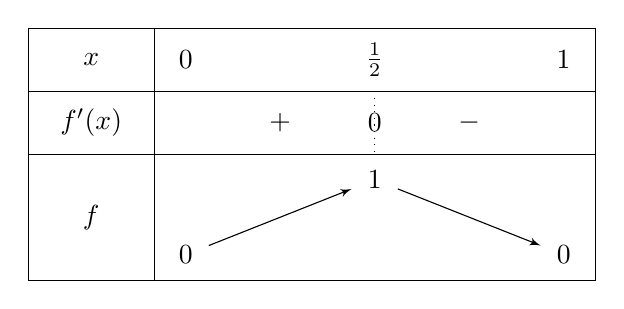
\begin{tikzpicture}[scale=0.8]
   \tkzTabInit{$x$ / 1 , $f'(x)$/1, $f$ / 2}{$0$, $\frac{1}{2}$,$1$}
   \tkzTabLine{,+,z, -, }
   \tkzTabVar{-/$0$,+/$1$,-/$0$}
\end{tikzpicture}\end{center}

En particulier, on voit que pour tout réel $x \in [0;1]$, on a $0 \leqslant f(x) \leqslant 1$. 

Pour tout entier naturel $n$, on pose $P(n)$ : « $0 \leqslant v_n\leqslant 1$ ».

\begin{itemize}
\item \textbf{Initialisation} : pour $n=0$, on a $v_0=0,3$ et donc $0 \leqslant v_n\leqslant 1$. $P(0)$ est vraie.
\item \textbf{Hérédité} : Soit $n\in\mathbb{N}$. Supposons que $P(n)$ est vraie, c'est-à-dire $0 \leqslant v_n\leqslant 1$. En utilisant les résultats de la question précédente, on a alors $0\leqslant f(v_n) \leqslant 1$, c'est-à-dire $0 \leqslant v_{n+1}\leqslant 1$. $P(n+1)$ est vraie.
\item \textbf{Conclusion} : $P(0)$ est vraie et $P$ est héréditaire. Par récurrence, $P(n)$ est vraie pour tout $n\in\mathbb{N}$.
\end{itemize}
\end{solution}


\newpage
\section*{Suites croissantes, suites décroissantes}



\begin{solution}Soit $n$ un entier naturel. On a
\[ u_{n+1}=2(n+1)^2-24(n+1)+3=2(n^2+2n+1)-24n-24+3\]
et donc
\[u_{n+1}=2n^2+4n+2-24n-24+3=2n^2-20n-19.\]
Ainsi,
\[ u_{n+1}-u_n = 2n^2-20n-19-(2n^2-24n+3)=4n-22.\]
Étudions le signe de $u_{n+1}-u_n$, c'est-à-dire le signe de $4n-22$. On a $4n-22 \geqslant 0$ si et seulement si $n \geqslant 5,5$. Ainsi, $(u_n)$ est décroissante jusqu'au rang 5 puis croissante à partir du rang 6. On a par ailleurs $u_5=-67$ et $u_6=-69$. Ainsi, $(u_n)$ est en fait décroissante jusqu'au rang 6 puis croissante à partir de ce rang. Une autre méthode consiste simplement à étudier les variations de la fonction $x\mapsto 2x^2-24x+3$.\end{solution}

\begin{exercise}
On considère la suite $(u_n)$ définie par $u_0=5$ et pour tout entier naturel $n$, $u_{n+1}=\dfrac{1}{2}u_n+4$.
\begin{enumerate}
\item Montrer par récurrence que, pour tout entier naturel $n$, $u_n \leqslant 8$.
\item Montrer que pour entier naturel $n$, $u_{n+1}-u_n = -\dfrac{1}{2}u_n+4$.
\item Déduire des deux questions précédentes que la suite $(u_n)$ est croissante.
\end{enumerate}\end{exercise}
\begin{solution}
Pour tout entier naturel $n$, on pose $P(n)$ : « $u_n \leqslant 8$ ».

\begin{itemize}
\item \textbf{Initialisation} : pour $n=0$, on a $u_0=5$ et donc $u_n \leqslant 8$. $P(0)$ est vraie.
\item \textbf{Hérédité} : Soit $n\in\mathbb{N}$. Supposons que $P(n)$ est vraie, c'est-à-dire $u_n \leqslant 8$. \\On a donc $\dfrac{1}{2}u_n+4 \leqslant \dfrac{1}{2}\times 8 +4$ c'est-à-dire $u_{n+1} \leqslant 8$. $P(n+1)$ est vraie.
\item \textbf{Conclusion} : $P(0)$ est vraie et $P$ est héréditaire. Par récurrence, $P(n)$ est vraie pour tout $n\in\mathbb{N}$.
\end{itemize}
Soit $n$ un entier naturel, on a $u_{n+1}-u_n = \dfrac{1}{2}u_n+4-u_n = -\dfrac{1}{2}u_n+4$.\\
Puisque pour tout entier naturel $n$, on a $u_n \leqslant 8$, on a donc $-\dfrac{1}{2}u_n \geqslant -\dfrac{1}{2} \times 8$ et $-\dfrac{1}{2}u_n+4 \geqslant -\dfrac{1}{2}\times 8 +4$, c'est-à-dire $u_{n+1}-u_n \geqslant 0$. La suite $(u_n)$ est donc croissante.\end{solution}

\begin{exercise}
On considère la suite \((u_n)\) définie par \(u_0=1\) et, pour tout entier naturel \(n\), \(u_{n+1}=\dfrac{2u_n}{2+u_n}\).
\begin{enumerate}
\item Montrer que pour tout entier naturel \(n\), \(u_n > 0\).
\item Montrer que la suite \((u_n)\) est strictement décroissante.
\end{enumerate}\end{exercise}

\begin{solution}Pour tout entier naturel \(n\), on pose \(P(n)\) : « \(u_n > 0\) ».

\begin{itemize}\item \textbf{Initialisation} : pour \(n=0\), on a \(u_0=1\) et donc \(u_0 > 0\). \(P(0)\) est vraie.
\item \textbf{Hérédité} : Soit \(n\in\mathbb{N}\). Supposons que \(P(n)\) est vraie, c'est-à-dire \(u_n > 0\). Or, \(u_{n+1}=\dfrac{2u_n}{2+u_n}\). \(u_{n+1}\) est donc le quotient de deux réels strictement positifs, il est donc strictement positif lui aussi. \(P(n+1)\) est vraie.
\item \textbf{Conclusion} : \(P(0)\) est vraie et \(P\) est héréditaire. Par récurrence, \(P(n)\) est vraie pour tout \(n\in\mathbb{N}\).
\end{itemize}
 On a montré que pour tout entier naturel \(n\), \(u_n > 0\). On peut donc déterminer les variations de la suite \((u_n)\) en étudiant le quotient \(\dfrac{u_{n+1}}{u_n}\). Or, pour tout entier naturel \(n\), 
\[\dfrac{u_{n+1}}{u_n} = \dfrac{2u_n}{2+u_n} \times \dfrac{1}{u_n} = \dfrac{2}{2+u_n}.\]
Or, puisque \(u_n > 0\), il en vient que \( 2+u_n > 2\) et donc que \( \dfrac{2}{2+u_n} < 1\). Ainsi, pour tout entier naturel \(n\), \(\dfrac{u_{n+1}}{u_n} < 1\), et donc \(u_{n+1} < u_n\). La suite \((u_n)\) est strictement décroissante.\end{solution}

\begin{exercise}
On considère la suite $(u_n)$ définie par $u_0=2$ et pour tout entier naturel $n$, $u_{n+1}=\dfrac{2}{3}u_n-7$. \\Montrer que pour tout entier naturel $n$, $u_n\geqslant -21$ et que la suite $(u_n)$ est décroissante.\end{exercise}


\begin{solution}
On rappelle qu'une suite décroissante vérifie que pour tout entier naturel $n$, $u_n \geqslant u_{n+1}$.

Pour tout entier naturel $n$, on pose $P(n)$ : « $u_n \geqslant u_{n+1} \geqslant -21$ ».

\begin{itemize}
\item \textbf{Initialisation} : pour $n=0$, on a $u_0=2$ et $u_1=\dfrac{2}{3}\times 2-7=-\dfrac{17}{3}$. On a bien  $u_0 \geqslant u_{1} \geqslant -21$. $P(0)$ est vraie.
\item \textbf{Hérédité} : Soit $n\in\mathbb{N}$. Supposons que $P(n)$ est vraie, c'est-à-dire $u_n \geqslant u_{n+1} \geqslant -21$.\\ On a donc $\dfrac{2}{3}u_n-7 \geqslant \dfrac{2}{3}u_{n+1}-7 \geqslant -21 \times \dfrac{2}{3} - 7$ c'est-à-dire $u_{n+1} \geqslant u_{n+2} \geqslant -21$. $P(n+1)$ est vraie.
\item \textbf{Conclusion} : $P(0)$ est vraie et $P$ est héréditaire. Par récurrence, $P(n)$ est vraie pour tout $n\in\mathbb{N}$.
\end{itemize}\end{solution}


\begin{exercise}
On considère la suite $(u_n)$ définie par $u_0=5$ et pour tout entier naturel $n$, $u_{n+1}=\sqrt{2u_n-1}$. \\Montrer que pour tout entier naturel $n$, $u_n \geqslant 1$ et que $(u_n)$ est décroissante.\end{exercise}


\begin{solution}
On rappelle qu'une suite décroissante vérifie que pour tout entier naturel $n$, $u_n \geqslant u_{n+1}$.

Pour tout entier naturel $n$, on pose $P(n)$ : « $u_n \geqslant u_{n+1} \geqslant 1$ ».

\begin{itemize}
\item \textbf{Initialisation} : pour $n=0$, on a $u_0=2=5$ et $u_1=\sqrt{2\times 5 -1}=\sqrt{9}=3$. On a bien  $u_0 \geqslant u_{1} \geqslant 1$. $P(0)$ est vraie.
\item \textbf{Hérédité} : Soit $n\in\mathbb{N}$. Supposons que $P(n)$ est vraie, c'est-à-dire $u_n \geqslant u_{n+1} \geqslant 1$.\\ On a donc $2u_n-1\geqslant 2u_{n+1}-1 \geqslant 2 \times 1 -1$. On applique alors la fonction $x\mapsto \sqrt{x}$ à l'inégalité. Cette fonction étant croissante sur $\mathbb{R}_+$, le sens de l'inégalité ne change pas. \\Ainsi, $\sqrt{2u_n-1} \geqslant \sqrt{2u_{n+1}-1} \geqslant \sqrt{2\times 1-1}$, c'est-à-dire $u_{n+1} \geqslant u_{n+2} \geqslant 1$.\\ $P(n+1)$ est vraie.
\item \textbf{Conclusion} : $P(0)$ est vraie et $P$ est héréditaire. Par récurrence, $P(n)$ est vraie pour tout $n\in\mathbb{N}$.
\end{itemize}\end{solution}

\begin{exercise}[subtitle={(Métropole 2021)}]
On considère la suite \((u_n)\) définie par \(u_0=1\) et, pour tout entier naturel \(n\),
\[u_{n+1}=\dfrac{5u_n+4}{u_n+2}.\]

\begin{enumerate}
\item Montrer que la fonction \(f\) définie pour tout réel \(x\in [0;+\infty [ \) par \(f(x)=\dfrac{5x+4}{x+2}\) est strictement croissante sur \([0,+\infty [\).
\item Montrer que pour tout entier naturel \(n\), 
\[ 0 \leqslant u_n \leqslant u_{n+1} \leqslant 4.\]
\end{enumerate}\end{exercise}
\begin{solution}La fonction \(f\) est dérivable comme quotient de fonctions dérivables sur \([0,+\infty [\), le dénominateur ne s'annulant pas sur cet intervalle. De plus, pour tout réel positif \(x\),
\[f'(x) = \dfrac{5 \times (x+2) - 1 \times (5x+4)}{(x+2)^2} = \dfrac{5x+10-5x-4}{(x+2)^2}=\dfrac{6}{(x+2)^2}.\]
Ainsi, pour tout réel positif \(x\), \(f'(x)> 0\). \(f\) est strictement croissante sur \([0;+\infty[\).

 Pour tout entier naturel \(n\), on considère la proposition \(\mathcal{P}(n)\) : « \(0 \leqslant u_n \leqslant u_{n+1} \leqslant 4\) ».
\begin{itemize} \item \textbf{Initialisation} : Pour \(n=0\), on a \(u_0=1\) et \(u_1 = \dfrac{5\times 1+4}{1+2} =\dfrac{9}{3}=3\) et donc \(0 \leqslant u_0 \leqslant u_1 \leqslant 4\). \(\mathcal{P}(0)\) est vraie.
\item \textbf{Hérédité} : Soit \(n\in\mathbb{N}\). Supposons que \(\mathcal{P}(n)\) est vraie, c'est-à-dire \(0 \leqslant u_n \leqslant u_{n+1} \leqslant 4\). 
La fonction \(f\) étant strictement croissante sur \([0;+\infty[ \), on peut l'appliquer à cette inégalité sans en changer le sens. Ainsi,
\[f(0) \leqslant f(u_n) \leqslant f(u_{n+1}) \leqslant f(4).\]
Or, \(f(0)=2\), qui est supérieur à 0, \(f(u_n)=u_{n+1}\), \(f(u_{n+1})=u_{n+2}\) et \(f(4)=4\). Il en vient que
\[0 \leqslant u_{n+1} \leqslant u_{n+2} \leqslant 4.\]
\(\mathcal{P}(n+1)\) est donc vraie.
\item \textbf{Conclusion} : \(\mathcal{P}(0)\) est vraie. \(\mathcal{P}\) est héréditaire. Par récurrence, \(\mathcal{P}(n)\) est vraie pour tout entier naturel \(n\).\end{itemize}\end{solution}



\begin{exercise}[subtitle={(Centres étrangers 2022)}]
On considère les suites \((a_n)\) et \((b_n)\) définies par \(a_0= \dfrac{1}{10}\), \(b_0=1\) et, pour tout entier naturel \(n\), \[\left\{\begin{array}{l}a_{n+1}=\mathrm{e}^{-b_n}\\b_{n+1}=\mathrm{e}^{-a_n}\end{array}\right.\]

On rappelle que la fonction \(x\mapsto e^{-x}\) est décroissante sur \(\mathbb{R}\). Montrer que pour tout entier naturel \(n\), 
\[ 0 < a_n \leqslant a_{n+1} \leqslant b_{n+1} \leqslant b_n \leqslant 1 .\]\end{exercise}

\begin{solution}Pour tout entier naturel \(n\), on pose \(P(n)\) : « \(0 < a_n \leqslant a_{n+1} \leqslant b_{n+1} \leqslant b_n \leqslant 1\) ».

\begin{itemize} \item \textbf{Initialisation} : pour \(n=0\), on a \(a_0=\dfrac{1}{10}\), \(b_0=1\), \(a_1 =\mathrm{e}^{-b_0}=\mathrm{e}^{-1}=\dfrac{1}{\mathrm{e}}\) et \(b_1=\mathrm{e}^{-a_0}=\mathrm{e}^{-0,1}\).

D'une part, puisque \( 10 \geqslant \mathrm{e}\), en appliquant la fonction inverse qui est décroissante sur \(\mathbb{R}^*_+\), on a que \(\dfrac{1}{10} \leqslant \dfrac{1}{\mathrm{e}}\), c'est-à-dire \(a_0 \leqslant a_1\). 

Par ailleurs, la fonction \(x \mapsto \mathrm{e}^{x}\) étant croissante sur \(\mathbb{R}\). On a donc que \(\mathrm{e}^{-1} \leqslant \mathrm{e}^{-0,1} \leqslant \mathrm{e}^0\), c'est-à-dire \(a_1 \leqslant b_1 \leqslant b_0\). 

Finalement, on a bien que \( 0< a_0 \leqslant a_1 \leqslant b_1 \leqslant b_0 \leqslant 1\). \(P(0)\) est donc vraie.

\item \textbf{Hérédité} : Soit \(n\in\mathbb{N}\). Supposons que \(P(n)\) est vraie, c'est-à-dire \(0 < a_n \leqslant a_{n+1} \leqslant b_{n+1} \leqslant b_n \leqslant 1\). La fonction \( x \mapsto \mathrm{e}^{-x}\) étant strictement décroissante sur \(\mathbb{R}\), on a alors 
\[\mathrm{e}^0 > \mathrm{e}^{-a_n} \geqslant \mathrm{e}^{-a_{n+1}} \geqslant \mathrm{e}^{-b_{n+1}} \geqslant \mathrm{e}^{-b_n} \geqslant \mathrm{e}^{-1}.\]

Ainsi, puisque \(\mathrm{e}^{-1} > 0\), on a, en lisant cette inégalité dans l'autre sens,
\[0 < a_{n+1} \leqslant a_{n+2} \leqslant b_{n+2} \leqslant b_{n+1} \leqslant 1.\]
\(P(n+1)\) est vraie.
\item \textbf{Conclusion} : \(P(0)\) est vraie et \(P\) est héréditaire. Par récurrence, \(P(n)\) est vraie pour tout \(n\in\mathbb{N}\).
\end{itemize}\end{solution}

\section*{Pour aller plus loin...}

\begin{exercise}[subtitle={(Suites arithmético-géométriques)}]

 Soit \(a\) et \(b\) deux réels, avec \(a\) différent de 0 et 1. On considère une suite \((u_n)\) telle que, pour tout \(n\in\mathbb{N}\), 
\[u_{n+1}=a\,u_n+b.\]
\begin{enumerate}
\item Résoudre l'équation \(x =ax+b\), d'inconnue réelle \(x\). On note \(r\) la solution de cette équation.
\item Montrer par récurrence que, pour tout entier naturel \(n\),
\[u_n=a^n(u_0-r)+r.\]
\item On propose de montrer ce résultat par une autre méthode. On considère pour cela la suite \((c_n)\) définie pour tout entier naturel \(n\) par \(c_n=u_n-r\).
\begin{enumerate}
\item Exprimer \(c_{n+1}\) en fonction de \(c_n\) pour tout entier naturel \(n\). 
\item Quelle est la nature de la suite \((c_n)\) ?
\item En déduire une expression de \(c_n\) puis de \(u_n\) en fonction de \(n\), pour tout entier naturel \(n\).\end{enumerate}\end{enumerate}\end{exercise}
\begin{solution}On a \(x=ax+b\) si et seulement si \(x-ax=b\) si et seulement si \(x(1-a)=b\) si et seulement si \(x=\dfrac{b}{1-a}\).

Pour tout entier naturel \(n\), on pose \(\mathcal{P}(n)\) : « \(u_n=a^n(u_0-r)+r\) ».
\begin{itemize} \item \textbf{Initialisation} : \(a^0 \times (u_0-r)+r = u_0-r+r=u_0\). \( \mathcal{P}(0) \) est vraie.
\item \textbf{Hérédité} : Soit \(n\) un entier naturel non nul. Supposons que \( \mathcal{P}(n)\) est vraie. On a donc \(u_n=a^n(u_0-r)+r\). Or,
\[u_{n+1}= au_n+b=a \times (a^n(u_0-r)+r) + b = a^{n+1} (u_0-r)+ar+b.\]
Or, \(r\) est solution de l'équation \(x =ax+b\). Ainsi, \(ar+b=r\). Il en vient que
\[u_{n+1}=a^{n+1} (u_0-r)+r.\]
\( \mathcal{P}(n+1)\) est donc vraie.
\item \textbf{Conclusion} : \(\mathcal{P}(0)\) est vraie et \(\mathcal{P}\) est héréditaire. Par récurrence, \(\mathcal{P}(n)\) est vraie pour tout \(n\in\mathbb{N}\).\end{itemize}

Pour tout entier naturel \(n\),
\[c_{n+1}=u_{n+1}-r=au_n+b-r\]
Or, \(r\) est solution de l'équation \(x=ax+b\). Ainsi,
\[c_{n+1}=au_n+b-(ar+b) =a(u_n-r)=a\times c_n.\]
La suite \((c_n)\) est une suite géométrique de raison \(a\).

D'après la question précédente, la suite \((c_n)\) est une suite géométrique de raison \(a\). Ainsi, pour tout entier naturel \(n\),
\[c_n=c_0 \times a^n = (u_0-r) \times a^n.\]
Or, pour tout entier naturel \(n\), \(c_n=u_n-r\) et donc \(u_n=c_n+r\). On en conclut que, pour tout entier naturel \(n\),
\[u_n=a^n(u_0-r)+r.\]\end{solution}


\begin{exercise}
On rappelle que pour tout entier naturel $n$, la fonction $f_n : x \mapsto x^n$, définie sur $\mathbb{R}$, est dérivable, de dérivée $f'_n : x \mapsto n\,x^{n-1}$. Nous allons le démontrer par récurrence.
\begin{enumerate}
\item Montrer, à l'aide du taux de variation, que les fonctions \(f_1 : x \mapsto x\) et \(f_2 : x \mapsto x^2\) sont dérivables sur \( \mathbb{R}\) et donner leur fonctions dérivées.
\item Soit $u$ et $v$ deux fonctions dérivables. Rappeler la formule de la dérivée de $uv$.
\item Pour tout entier naturel $n$, on pose $\mathcal{P}(n)$ la proposition « $f_n$ est dérivable sur $\mathbb{R}$ et pour tout réel $x$, $f'_n(x)=n\,x^{n-1}$ ». Démontrer cette proposition par récurrence.\end{enumerate}
\end{exercise}

\begin{solution} Pour tout réel \(x\) et tout réel non nul \(h\),
\[ \dfrac{f_1(x+h) - f_1(x)}{h}=\dfrac{x+h-x}{h} = \dfrac{h}{h}=1.\]

Ainsi, \(f_1\) est dérivable sur \(\mathbb{R}\) et pour tout réel \(x\), \(f'_1(x)=1\). Par ailleurs, pour tout réel \(x\) et tout réel \(h\) non nul,
\[\dfrac{f_2(x+h)-f_2(x)}{h}=\dfrac{(x+h)^2-x^2}{h}=\dfrac{x^2+2hx+h^2-x^2}{h}=2x+h.\]

Ainsi, \(f_2\) est dérivable sur \(\mathbb{R}\) et pour tout réel \(x\), \(f'_2(x)=2x\).

Soit \(u\) et \(v\) deux fonctions dérivables sur \(\mathbb{R}\). Alors \(uv\) est dérivable sur \(\mathbb{R}\) et \((uv)'=u'v+uv'\).

Pour tout entier naturel \(n\) supérieur ou égal à 2, on considère la proposition \( \mathcal{P}(n)\) : « la fonction \(f_n : x \mapsto x^n\) est dérivable sur \(\mathbb{R}\), de dérivée \(f'_n : x \mapsto nx^{n-1}\) ».
\begin{itemize} \item \textbf{Initialisation} : D'après la question 1., \(f_2\) est dérivable sur \(\mathbb{R}\) et pour tout réel \(x\), \(f'_2(x)=2x=2x^{2-1}\). \(\mathcal{P}(2)\) est donc vraie.
\item \textbf{Hérédité} : Soit \(n\) un entier naturel supérieur ou égal à 2. Supposons que \( \mathcal{P}(n)\) est vraie. Pour tout réel \(x\)\[ f_{n+1}(x) = x^{n+1} = x \times x^n = f_1(x) \times f_n(x) .\]
Or, \(f_1\) est dérivable sur \(\mathbb{R}\) (question 1.) et \(f_n\) est également dérivable sur \(\mathbb{R}\) par hypothèse de récurrence. Ainsi, \(f_{n+1}\) est dérivable sur \(\mathbb{R}\) et
\[f'_{n+1}=f'_1 \times f_n + f_1 \times f'_n.\]
Pour tout réel \(x\),
\[ f'_{n+1}(x)= 1 \times x^n + x \times n\,x^{n-1} = x^n+n\,x^n=(n+1)x^n=(n+1) x^{n+1-1}.\]
\(\mathcal{P}(n+1)\) est donc vraie.
\item \textbf{Conclusion} : \(\mathcal{P}(2)\) est vraie et \(\mathcal{P}\) est héréditaire. Par récurrence, \(\mathcal{P}(n)\) est vraie pour tout entier naturel \(n\) supérieur ou égal à 2\end{itemize}\end{solution}

\begin{exercise}La suite de Fibonacci est la suite $(F_n)$ définie par $F_0=F_1=1$ et, pour tout entier naturel $n$, $F_{n+2}=F_{n+1}+F_n$.

Pour tout entier naturel $n$, on note $\Delta_n=F_nF_{n+2}-F_{n+1}^2$.

Conjecturer une expression de $\Delta_n$ en fonction de $n$ puis démontrer cette conjecture par récurrence.\end{exercise}

\begin{exercise}Pour tout entier naturel non nul $n$, on note $n!$ l'entier défini par $n! = 1 \times 2 \times \ldots \times n$.\\ On convient par ailleurs que $0!=1$.

Montrer que pour tout entier naturel $n$ et tout réel $x\geqslant 0$, on a
\[\exp(x)\geqslant 1 + x + \dfrac{x^2}{2!}+\dfrac{x^3}{3!}+\ldots + \dfrac{x^n}{n!}\]\end{exercise}

\chapter{Correction des exercices}

\printsolutions[headings={false}]

\end{document}